
% !TEX encoding = UTF-8 Unicode 
% !TEX root = FieldGuide.tex

\Sec{Grand Unified Distribution}
\label{sec:GUD}



The Grand Unified Distribution of order $n$ is required to satisfy the following differential equation.
\begin{align}
\label{GUD}
\frac{d}{dx} \ln  \opr{GUD}^{(n)}&(x\given a, s \sep a_0, a_1,\ldots,a_n\sep  b_0,b_1,\ldots, b_n\sep \beta)
\checked \\
&= -\Left|\tfrac{\beta}{s}\Right| \frac{1}{\bigl(\tfrac{x-a}{s}\bigr)} \frac{a_0  +a_1 \bigl(\tfrac{x-a}{s}\bigr)^{\beta}+\cdots +a_n \bigl(\tfrac{x-a}{s}\bigr)^{n\beta}}{b_0+ b_1 \bigl(\tfrac{x-a}{s}\bigr)^{\beta}+\cdots+b_n\bigl(\tfrac{x-a}{s}\bigr)^{n\beta}  } 
\notag
\checked
\\
& \qquad  a,\ s,\  a_0,a_1,\ldots,a_n,\ b_0,b_1, \ldots, b_n,\ \beta,\ x\  \text{ in } \mathbb{R} 
\checked
\notag
\\ \notag
& \qquad \beta = 1 \text{ when } a_0 =0
\checked
\end{align}
In principal, any analytic probability distribution can satisfy this relation.
The central hypothesis of this compendium is that most interesting univariate continuous probability distributions satisfy this relation with low order polynomials in the denominator and numeration. If fact, there seems be little need to consider beyond $n=2$, which we take as the default order, in the absence of further qualification. 



\SSec{Special cases}

\dist{Extended Pearson} distribution~\cite{Roy1971}: With $\beta=1$ we obtain an extended Pearson distribution.
\begin{align}
\label{ExtPearson}
&\frac{d}{dx} \ln  \opr{ExtPearson}(x\given 0, 1\sep a_0, a_1, a_2\sep b_0, b_1, b_2) \checked \\
\notag
&= - \frac{1}{x} \frac{a_0 +a_1 x+ a_2 x^2}{b_0+ b_1 x+  b_2 x^2  } \\
\notag
& a,\ s,\ a_0,\ a_1,\ a_2,\ b_0,\ b_1,\ b_2 \text{ in } \Real
\end{align}



\begin{figure*}
\thispagestyle{chapter}
\caption[Grand Unified Distributions]{Grand Unified Distributions} 
\begin{center}
\scalebox{0.6} {
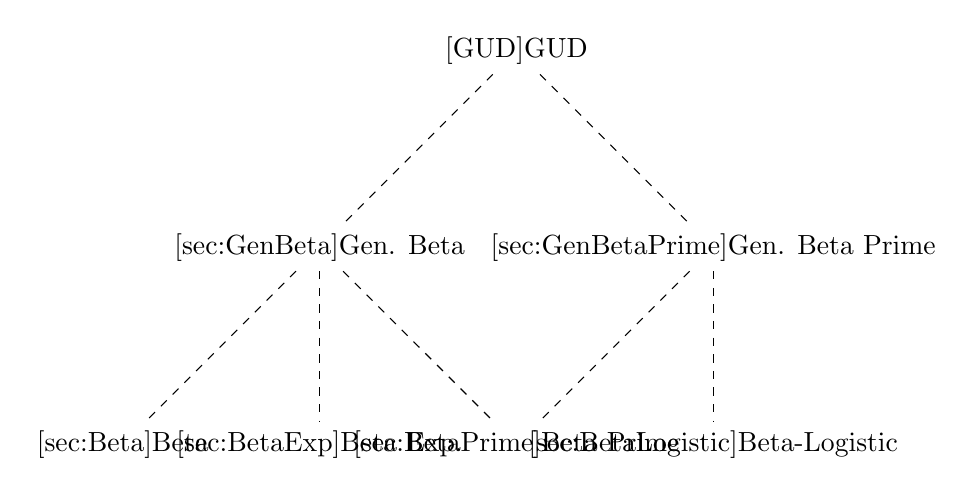
\begin{tikzpicture}
%\draw[help lines, very thin, step=1] (-2,0) grid (17,17);
%
%\draw (7.5,16.75) node (ExtPearson) {\hyperref[ExtPearson]{Ext. Pearson}};
%%\draw (7.5,15) node (PearsonExp) {\hyperref[PearsonExp]{Pearson Exp.}};
%\draw (7.5,16.75) node (ExtPearson) {\hyperref[ExtPearson]{Ext. Pearson}};

\draw (7.5,17.5) node (gud) {\hyperref[GUD]{GUD}};
%
\draw (5,15) node (genbeta) {\hyperref[sec:GenBeta]{Gen. Beta}};
%\draw (7.5,15) node (pearson) {\hyperref[sec:Pearson]{Pearson}};
\draw (10,15) node (genbetaprime) {\hyperref[sec:GenBetaPrime]{Gen. Beta Prime}};
%
\draw (2.5,12.5) node (beta) {\hyperref[sec:Beta]{Beta}};
\draw (5,12.5) node (betaexp) {\hyperref[sec:BetaExp]{Beta Exp.}};
\draw (7.5,12.5) node (betaprime) {\hyperref[sec:BetaPrime]{Beta Prime}};
\draw (10,12.5) node (betalogistic) {\hyperref[sec:BetaLogistic]{Beta-Logistic}};
%\draw (12.5,12.5) node (pearsoniv) {\hyperref[sec:PearsonIV]{Pearson IV}};
%
%\draw (2.5,10) node (unitgamma) {\hyperref[sec:UnitGamma]{Unit Gamma}};
%\draw (7.5,10) node (amoroso) {\hyperref[sec:Amoroso]{Amoroso}};
%\draw (12.5,10) node (burr) {\hyperref[Burr]{Burr}};
%
\draw [dashed]  (gud) -- (genbeta);
%\draw [dashed]  (gud) -- (pearson);
\draw [dashed]  (gud) -- (genbetaprime);
%%\draw [dashed]  (gud) -- (PearsonExp);
%%\draw [dashed]  (PearsonExp) -- (betaexp);
%%\draw [dashed]  (PearsonExp) -- (betalogistic);
%
\draw [dashed]  (genbeta) -- (beta);
\draw [dashed]  (genbeta) -- (betaexp);
\draw [dashed]  (genbeta) -- (betaprime);
%\draw [dashed]  (genbeta) -- (unitgamma);
%\draw [dashed]  (genbeta) -- (amoroso);
%
%\draw [dashed]  (pearson) -- (beta);
%\draw [dashed]  (pearson) -- (betaprime);
%\draw [dashed]  (pearson) -- (pearsoniv);
%
\draw [dashed]  (genbetaprime) -- (betalogistic);
\draw [dashed]  (genbetaprime) -- (betaprime);
%\draw [dashed]  (genbetaprime) -- (amoroso);
%\draw [dashed]  (genbetaprime) -- (burr);
%
%\draw[|-|, very thin] (-1.5,0.5) -- node[fill=white, midway] {0} (-1.5,3);
%\draw[|-|, very thin]  (-1.5,4.5) -- node[fill=white, midway] {1} (-1.5,8);
%\draw[|-|, very thin]  (-1.5,9.5) -- node[fill=white, midway] {2} (-1.5,13);
%\draw[|-|, very thin]  (-1.5,14.5) -- node[fill=white, midway] {3} (-1.5,15.5);
%\draw[|-|, very thin]  (-1.5,16) -- node[fill=white, midway] {4} (-1.5,17);
%
%
%\draw (-1, 15.75) node[rotate=90]  {\small shape parameters};
%
%\draw[white] (-2, 0) rectangle (17,17.5); % Bounding box
\end{tikzpicture}
}
\end{center}
\end{figure*}




\begin{table*}[bp]
\begin{center}
\caption[Grand Unified Distribution -- Special cases]{Special cases of the Grand Unified Distribution}
~\\
{\renewcommand{\arraystretch}{1.25} 
\begin{tabular}{llcccccccccc}
\eqref{GUD}  & GUD & $a$ & $s$ & $a_0$ & $a_1$ & $a_2$ & $b_0$ & $b_1$ & $b_2$  & $\beta$ \\
\hline
\eqref{ExtPearson} & Ext.\ Pearson  &.&.&.&.&.&.&.&.&$1$ \checked\\
\eqref{Pearson}	 & Pearson  &.&.&0&.&.&.&.&.&$1$ \checked\\
\eqref{GenBeta} & gen.\ beta &.&.&.&.&0&0&1&-1&. \checked\\
\eqref{GenBeta} & gen.\ beta prime &.&.&.&.&0&0&1&1&. \checked\\
\eqref{InvGaussian}	 & inv.\ Gaussian &.&.&.&$\tfrac{3}{2}$&.&0&1&0&1 \checked \\
\eqref{RecInvGaussian}   & rec.\ inv.\ Gaussian$\!\!\!\!$ &.&.&.&$\tfrac{3}{2}$&.&0&1&0&-1 \\
\eqref{Halphen} & Halphen &.&.&$-\kappa$&$1$-$\alpha$&$\kappa$&0&1&0&1 \checked \\
\eqref{GenHalphen} & gen.\ Halphen &.&.&$-\kappa$&$1$-$\alpha$&$\kappa$&0&1&0&$\beta$ \\
\eqref{Hyperbola} & Hyperbola &.&.&$-\kappa$&1&$\kappa$&0&1&0&1 \checked \\
\eqref{HalphenB} & Halphen B&.&.&$1$-$\alpha$&$-\kappa$&$2$ &1&0&0 &1  \\
\eqref{InvHalphenB} & inv.\ Halphen B&.&.&-2&$-\kappa$&$\!\!1$-$\alpha$&0&1&0&1 \checked \\
\eqref{Sichel} & Sichel &.&.&$-\lambda$&$1$-$\alpha$&$\kappa$&0&1&0&1 \checked \\
\eqref{GenSichel} & gen.\ Sichel &.&.&$-\lambda$&$1$-$\alpha$&$\kappa$&0&1&0&$\beta$ \\
\end{tabular} 
}
\end{center}
\end{table*}


%===========================================================================
\dist{Inverse Gaussian} (Wald, inverse normal) distribution~\cite{Wald1944,Tweedie1945,Folks1978,Chhikara1989,Johnson1994}: 
\begin{align}
\label{InvGaussian}
\opr{InvGaussian}(x\given \mu,\lambda) &= \sqrt{\frac{\lambda}{2\pi x^3}} \exp\Left(\frac{-\lambda (x-\mu)^2}{2\mu^2 x}\Right) \checked
\\ \notag
& = \opr{ExtPearson}(x\given 0,1 \sep -\tfrac{\lambda}{2}, \tfrac{3}{2}, \tfrac{\lambda}{2\mu^2} \sep 0, 1,0) \checked
\\ \notag
& = \opr{GUD}(x\given 0,1 \sep -\tfrac{\lambda}{2}, \tfrac{3}{2}, \tfrac{\lambda}{2\mu^2} \sep  0, 1,0 \sep 1) \checked
\end{align}
with support $x>0$, mean $\mu>0$, and shape $\lambda>0$. The name `inverse Gaussian' is misleading, since this is not in any direct sense the inverse of a Gaussian distribution. 
The {\bf Wald} distribution is a special case with $\mu=1$.
% D[-Log[sqrt(L /(2 pi x^3)) exp(-{L(x- m)^2} / {2m^2 x})], x]

The inverse Gaussian distribution describes first passage time in one dimensional Brownian diffusion with drift~\cite{Chhikara1989}. The displacement $x$ of a diffusing particle after a time $t$, with diffusion constant $D$ and drift velocity $v$,  is $\opr{Normal}(vt, \sqrt{2 D t})$. The `inverse' problem is to ask for the first passage time, the time taken to first reach a particular position $y>0$, which is distributed as $\opr{InvGaussian}(\tfrac{y}{v},\tfrac{y^2}{2D})$. \index{first passage time}\index{diffusion}

In the limit that $\mu$ goes to infinity we recover the L\'evy distribution \eqref{Levy}, the first passage time distribution for Brownian diffusion without drift.
\[
\lim_{\mu\rightarrow\infty} \opr{InvGaussian}(x\given \mu, \lambda) = \Levy(x\given 0,\lambda) \checked
\notag
\]

The sum of independent inverse Gaussian random variables is also inverse Gaussian, provided that $\mu^2/\lambda$ is a constant.
\begin{align*}
\sum_i \opr{InvGaussian}_i &(x\given \mu' w_i, \lambda' w_i^2)
\\
& \sim \opr{InvGaussian}\Bigl(x\given \mu' \sum_i w_i, \lambda' \bigl(\sum_i w_i\bigr)^2 \Bigr) \checked
\end{align*}

Scaling an inverse Gaussian scales both $\mu$ and $\lambda$. 
\[
c\ \opr{InvGaussian} (\mu, \lambda) \sim \opr{InvGaussian} (c \mu, c \lambda) \checked
\notag
\]

It follows from the previous two relations the sample mean of an inverse Gaussian is inverse Gaussian.
\[
\frac{1}{N} \sum_{i=1}^N \opr{InvGaussian}_i (\mu, \lambda) \sim \opr{InvGaussian} (\mu, N \lambda) \checked
\notag 
\]



\dist{Reciprocal inverse Gaussian} distribution~\cite{Johnson1994}: 
\begin{align}
\label{RecInvGaussian}
\opr{RecInvGaussian}(x\given \mu,\lambda) &= \sqrt{\frac{\lambda}{2\pi x}} \exp\Left(\frac{-\lambda (1-\mu x)^2}{2\mu^2 x}\Right) \checked
\\ \notag
& = \opr{ExtPearson}(x\given 0,1 \sep -\tfrac{\lambda}{2\mu^2}, \tfrac{1}{2}, \tfrac{\lambda}{2} \sep 0, 1,0) \checked
\\ \notag
& = \opr{GUD}(x\given 0,1 \sep -\tfrac{\lambda}{2}, \tfrac{3}{2}, \tfrac{\lambda}{2\mu^2} \sep 0, 1,0 \sep -1) \checked
\end{align}
with support $x>0$, mean $\mu>0$, and shape $\lambda>0$. An inverted (in standard sense) inverse Gaussian distribution. 
\[
\opr{RecInvGaussian}(\mu,\lambda) \sim \opr{InvGaussian}(\mu,\lambda)^{-1}
\notag
\]
% D[-Log[sqrt(L /(2 pi x)) exp(-{L(1- m x)^2} / {2m^2 x})], x]



\dist{Halphen} (Halphen A) distribution~\cite{Halphen1941}:
\begin{align}
\label{Halphen}
&\opr{Halphen}(x\given a,s, \alpha, \kappa)
\\
&= \frac{1}{2 |s| K_{\alpha} (2\kappa)} \Left(\frac{x-a}{s}\Right)^{\alpha-1} 
\exp\Left\{-\kappa \Left(\frac{x-a}{s}\Right) -\kappa \Left(\frac{x-a}{s}\Right)^{-1}\Right\},
\checked
\notag
\\
 &=  \op{GUD}(x\given a,s \sep -\kappa, 1-\alpha, \kappa\sep 0,1,0 \sep 1)
\notag
\checked
\\& \qquad  0 \leq \tfrac{x-a}{s}
\notag
\end{align}
Developed by \'Etienne Halphen for the frequency analysis of river flows.
Limits to gamma, inverse gamma, and normal.



% D[log(x^{(-1)} e^{-k x -k/x}),x]
% D[log(x^{(a-1)} e^{-k x -k/x}),x]
% Halphen B: D[-log(x^{(a-1)} e^{-x^2 +k x}),x]
% Inv. Halphen B:  D[-log(x^{(a-1)} e^{-x^(-2) +k / x}),x] 
% Sichel: D[log(x^{(a-1)} e^{-k x -L/x}),x]
\dist{Hyperbola} (harmonic) distribution~\cite{Halphen1941,Perreault1999}:
\begin{align}
\label{Hyperbola}
&\opr{Hyperbola}(x\given a,s,\kappa)
\\ 
&= \frac{1}{2 |s| K_0(2\kappa)} \Left(\frac{x-a}{s}\Right)^{-1} 
\exp \Left\{ -\kappa \Left(\frac{x-a}{s}\Right) -\kappa \Left(\frac{x-a}{s}\Right)^{-1} \Right\},
\checked
\notag
\\
& = \op{Halphen}(x\given a,s, 0, \kappa)
\checked
\notag
\\
& = \op{GUD}(x\given a,s\sep -\kappa, 1 , \kappa\sep 0,1,0\sep 1)
\checked
\notag
\\& \qquad  0 \leq \tfrac{x-a}{s}
\notag
\end{align}




\dist{Halphen B} distribution~\cite{Halphen1941,Perreault1999}:
\begin{align}
\label{HalphenB}
&\opr{HalphenB}(x\given a,s, \alpha, \kappa)
\\
&= \frac{2}{|s| H_{2 \alpha}(\kappa)} \Left(\frac{x-a}{s}\Right)^{\alpha-1} 
\exp\Left\{- \Left(\frac{x-a}{s}\Right)^{2} +\kappa \Left(\frac{x-a}{s}\Right)\Right\},
\checked
\notag
\\
& = \op{GUD}(x\given a,s\sep 1-\alpha, -\kappa,  2\sep 1,0,0\sep 1) \checked
\notag
\\& \qquad  0 \leq \tfrac{x-a}{s}
\notag
\end{align}
The normalizing function $H_{2 \alpha}(\kappa)$ was called the exponential factorial function by Halphen~\cite{Halphen1955a, Perreault1999}.
Limits to gamma distribution \eqref{Gamma} as $\kappa \rightarrow \infty$.
\index{exponential factorial function}

% According to Perreault1999, cite Morlat1956a not Halphen1941
\dist{Inverse Halphen B} distribution~\cite{Morlat1956a,Perreault1999}:
\begin{align}
\label{InvHalphenB}
&\opr{InvHalphenB}(x\given a,s, \alpha, \kappa)
\\
&= \frac{2}{|s| H_{2\alpha}(\kappa)} \Left(\frac{x-a}{s}\Right)^{-\alpha+1} 
\exp\Left\{- \Left(\frac{x-a}{s}\Right)^{-2} +\kappa \Left(\frac{x-a}{s}\Right)^{-1}\Right\},
\checked
\notag
\\
& = \op{GUD}(x \given a,s\sep -2, -\kappa, 1-\alpha\sep 0,0,1\sep1) \checked
\notag
\\& \qquad  0 \leq \tfrac{x-a}{s}
\notag
\end{align}
Limits to inverse gamma distribution \eqref{InvGamma} as $\kappa \rightarrow \infty$.

\dist{Sichel} (generalized inverse Gaussian) distribution~\cite{Good1953, Sichel1973, Barndorff-Nielsen1977}:
\begin{align}
\label{Sichel}
&\opr{Sichel}(x\given a,s, \alpha, \kappa, \lambda)
\\
&= \frac{(\kappa/\lambda)^{\alpha/2} }{2 |s| K_{\alpha} (2\sqrt{\kappa\lambda})} \Left(\frac{x-a}{s}\Right)^{\alpha-1} 
\exp\Left\{-\kappa \Left(\frac{x-a}{s}\Right) -\lambda \Left(\frac{x-a}{s}\Right)^{-1}\Right\},
\notag
\checked
\\
& = \op{GUD}(x \given a,s \sep -\lambda, 1-\alpha , \kappa \sep 0,1,0 \sep 1)
\notag
\\& \qquad  0 \leq \tfrac{x-a}{s} \notag
\end{align}
Special cases include Halphen \eqref{Halphen} $\lambda= \kappa$, and inverse Gaussian \eqref{InvGaussian} $\alpha = -\tfrac{1}{2}$.




\dist{Libby-Novick} distribution~\cite{Libby1982a, McDonald1995, Sarabia2006, Nadarajah2007}
\begin{align}
\label{LibbyNovick}
&\opr{LibbyNovick}(x\given a,s,c,\alpha,\gamma)
\\ \notag
&=  \frac{1}{|s| B(\alpha,\gamma)}
\Left(\tfrac{x-a}{s}\Right)^{\alpha-1}  \Left(1-\tfrac{x-a}{s}\Right)^{\gamma-1} \Left(1- (1-c) \tfrac{x-a}{s}\Right)^{-\alpha-\gamma}
\checked
\notag
\\ \notag
& = \op{GUD}(x\given a,s\sep \alpha-1, 3-\alpha - c - c\gamma, 2c-2\sep
\\ \notag & \qquad\qquad\qquad 1, c-2, 1-c\sep 1) \checked
\\ \notag
& \qquad \text{for } a,s,c,\alpha,\gamma  \text{ in } {R},  \alpha,\gamma  >0
\\ \notag
& \qquad 0\leq \tfrac{x-a}{s} \leq1
\end{align}
A generalized three-parameter beta distribution that arises naturally as a beta distribution style ratio of gamma distributions~\cite{Sarabia2006}. 
\[
\opr{LibbyNovick}(0, \tfrac{s_1}{s_2}, \alpha, \gamma) \sim \frac{\opr{Gamma}_1(0, s_1,\alpha)} { \opr{Gamma}_1(0, s_1,\alpha) + \opr{Gamma}_2(0, s_2,\gamma) }
\notag
\checked
\]
Limits to both the beta ($u=1$) and beta-prime ($u\rightarrow \infty$ ) distributions. 
% D[Log[x^(a-1)(1-x)^(g-1)(1-(1-u)x)^(-a-g)], x]

\dist{Gauss hypergeometric} distribution~\cite{Armero1994,Sarabia2006}
\begin{align}
\label{GaussHypergeometric}
&\opr{GaussHypergeometric}(x\given a,s,u, \alpha, \gamma, \delta)
\\ \notag
& =   \frac{1}{|s| \mathcal{N}} 
\Left(\frac{x-a}{s}\Right)^{\alpha-1}  \Left(1-\frac{x-a}{s}\Right)^{\gamma-1} \Left(1- (1-u) \frac{x-a}{s}\Right)^{-\delta}
\checked
\notag
\\ \notag
& \quad \mathcal{N} = B(\alpha,\gamma)\  {}_2F_1(\alpha,\delta;\alpha+\gamma,1-u) \checked
\\ \notag
& \qquad \text{for } a, s, u,\alpha,\gamma, \delta  \text{ in } \mathbb{R},  \alpha,\gamma, \delta >0
\\ \notag &
=\op{GUD}(x\given a, s \sep \alpha-1,2 - \alpha -\gamma + (1-u)(1+ \rho+\alpha), \checked \\
& \qquad\qquad \qquad\notag
u(\alpha+\gamma-\rho-2) \sep 1, -1-c, -u \sep 1)
\\ \notag
& \qquad 0\leq \tfrac{x-a}{s} \leq1
\end{align}
% A natural generalization of the three-beta distribution. 
Motivated by the Euler integral formula for the Gauss hypergeometric function~\secref{sec:math}. 


\dist{Confluent hypergeometric} distribution~\cite{Gordy1988a,Nadarajah2006a,Nadarajah2007}
\begin{align}
\label{Confluent}
\opr{Confluent}&(x \given \alpha, \gamma, \delta) 
\\& =
\notag
\frac{1}{\mathcal{N}}  
\Left(\frac{x-a}{s}\Right)^{\alpha-1} \Left(1- \Left(\frac{x-a}{s}\Right)\Right)^{\gamma-1} \exp\Left\{-\kappa \Left(\frac{x-a}{s}\Right)\Right\} \checked
\notag
\\
& \qquad \mathcal{N} = B(\alpha, \gamma)\ {}_1 F_1(\alpha; \alpha+\gamma; -\kappa)
\notag 
\\
&= \op{GUD}(x\given 0,1 \sep 1-\alpha, \alpha+\gamma+\kappa -2, -\kappa \sep 1,-1,0 \sep 1) \checked
\notag
\\
& \qquad0 \leq \tfrac{x-a}{s} \leq 1 \notag
\end{align}
This distribution was introduced by Gordy~\cite{Gordy1988a} for applications to auction theory.
% D[Log[ x^(a-1) (1-x)^(g-1) Exp[-k x] ] , x]
% Add location and scale 




%\SSec{Special cases: \texorpdfstring{$\beta\neq1$}{beta neq 1}}


\dist{Generalized Halphen}~\cite{\self} :
\begin{align}
\label{GenHalphen}
&\opr{GenHalphen}(x\given a,s, \alpha, \kappa, \beta) 
\\
&= \frac{|\beta|}{2 |s| K_{\alpha} (2\kappa)} \Left(\frac{x-a}{s}\Right)^{\beta \alpha-1} 
\exp\Left\{-\kappa \Left(\frac{x-a}{s}\Right)^\beta -\kappa \Left(\frac{x-a}{s}\Right)^{-\beta}\Right\}  \checked
\notag
\\
& = GUD(x\given a,s\sep -\kappa, 1-\alpha , \kappa\sep 0,1,0\sep\beta) \checked
\notag
\\
& \qquad0 \leq (\tfrac{x-a}{s})^\beta \notag
\end{align}


\dist{Generalized Sichel} (generalized generalized inverse Gaussian) distribution~\cite{Shakil2010a}:
\begin{align}
\label{GenSichel}
&\opr{GenSichel}(x\given a,s, \alpha, \kappa, \lambda, \beta)
\\
&= \frac{|\beta| (\kappa/\lambda)^{\alpha/2} }{2 |s| K_{\alpha} (2\sqrt{\kappa\lambda})} \Left(\frac{x-a}{s}\Right)^{\beta\alpha-1}
\exp\Left\{-\kappa \Left(\frac{x-a}{s}\Right)^\beta -\lambda \Left(\frac{x-a}{s}\Right)^{-\beta}\Right\}, \checked
\notag
\\
& = \op{GUD}(x \given a,s \sep -\lambda, 1-\alpha , \kappa \sep 0,1,0 \sep \beta) \checked
\notag
\\& \qquad  0 \leq  (\tfrac{x-a}{s})^\beta \notag
\end{align}
Special cases include the generalized Halphen \eqref{GenHalphen} $\lambda= \kappa$, and Sichel \eqref{Sichel} distributions $\beta = 1$.




\pagebreak[4]

\begin{table*}[tp]
\begin{center}
\caption[Pearson-exponential distributions -- Special cases]{Special cases of the Pearson exponential family}
~\\
\label{PearsonExpTable}
\begin{tabular}{llcccccccccc}
\eqref{PearsonExp}  & Pearson Exp. & $\pLoc$ & $\pScale$ & $a_0$ & $a_1$ & $a_2$ & $b_0$ & $b_1$ & $b_2$  \\
% 
\hline
\eqref{BetaExp} & beta-exp.  &.&.&0&$\alpha$+$\gamma$-$1$&-$\alpha$  &0&1&-1\\ %D[-Log[Exp(- a x) (1 - Exp(-x) )^(g-1) ],x]
\eqref{BetaLogistic} & beta-logistic    &.&.&0&-$\gamma$&$\alpha$  &0&1&1 \\ % D[Log[ Exp(- a x) (1 + Exp(-x) )^(-a-g) ],x]
\eqref{CentralLogistic} & central-logistic    &.&.&0&-$\alpha$&$\alpha$  &0&1&1 \\
\eqref{Perks} & Perks    &.&.&-1&0&1&1&$c$&1 \\
\eqref{Logistic} & logistic     &.&.&0&-1&1  &0&1&1 \\
\eqref{HyperbolicSecant} & hyperbolic secant     &.&.&0&-\half&\half  &0&1&1\\
\eqref{GammaExp} & gamma exp.    &.&.&0&-$\alpha$&1&0&1&0 \\
\eqref{Exp} & exponential    &.&.&0&1&0&0&1&0
\end{tabular} 
\end{center}
\end{table*}
\todo{Table of Person Exponential}


\SSec{Pearson-exponential distributions}

If we take the limit of $\beta$ to infinity (See \secref{sec:Limits:exp}), then we get the family of Pearson exponential distributions.

\dist{Pearson-exponential} distribution~\cite{\self}:
\begin{align}
\opr{PearsonExp}&(x\given  \pLoc, \pScale \sep a_0, a_1,a_2 \sep  b_0,b_1,b_2)
 \label{PearsonExp}
  \\ &= \lim_{\beta\rightarrow \infty} \opr{GUD}(x\given \pLoc + \beta \pScale, \beta \pScale\sep a_0, a_1,a_2\sep  b_0,b_1,b_2\sep \beta) 
\notag
\end{align}

Because we can generally interchange limits and differentiation, such distributions satisfy the following differential equation.
\begin{align}
\frac{d}{dx} \ln \opr{PearsonExp}&(x\given  \pLoc, \pScale \sep a_0, a_1,a_2\sep  b_0,b_1,b_2) 
\notag
\\
&= \left|\tfrac{1}{\lambda}\right|  \frac{a_0  +a_1 e^{\tfrac{x-\pLoc}{\pScale}} +a_2 e^{2\tfrac{x-\pLoc}{\pScale}} }
{b_0+ b_1 e^{\tfrac{x-\pLoc}{\pScale}}+b_2 e^{2\tfrac{x-\pLoc}{\pScale} }}
\notag
\end{align}
See table~\ref{PearsonExpTable} and Fig.~\ref{PearsonExpHierarchy}.


\dist{Perks} (Champernowne) distribution~\cite{Perks1932,Champernowne1952,Talacko1956,Devroye1986}:
\begin{align}
\label{Perks}
\opr{Perks}(x\given \pLoc, \pScale, c)
&= \frac{1}{\mathcal{N}} \frac{1}{c + e^{-\tfrac{x-\pLoc}{\pScale}} + e^{+\tfrac{x-\pLoc}{\pScale}}} \checked
\\
& = \op{PearsonExp}(x \given \pLoc, \pScale \sep -1, 0 , -1 \sep 1, c, 1) \checked
\notag
\end{align}
Special cases include logistic ($c=0$) \eqref{Logistic} and 
hyperbolic secant ($c=2$) \eqref{HyperbolicSecant} distributions.





\SSec{Greater Grand Unified distributions}

There are only a few interesting specials cases of the Grand Unified Distribution with order greater than 2.


%===========================================================================
\dist{Appell Beta} distribution~\cite{Nadarajah2006a}:
\begin{align}
\label{AppellBeta}
&\op{AppellBeta}(x \given a,s, \alpha, \gamma, \rho, \delta) \notag
\\& \qquad= \frac{1}{\mathcal{N}\ |s|} 
\frac{ \bigl(\frac{x-a}{s}\bigr)^{\alpha-1} \bigl(1-\frac{x-a}{s}\bigr)^{\gamma-1} }
	{ \bigl(1 - u \frac{x-a}{s} \bigr)^{\rho} \bigl(1-v \frac{x-a}{s} \bigr)^{\delta} }
	\checked
\\
&\qquad \mathcal{N}  = B(\alpha, \gamma)\ F_1(\alpha,\rho,\delta,\alpha+\gamma;  u, v)\checked
\notag
\\ \notag
&= \op{GUD}^{(3)}(x\given a,s \sep a_0,a_1,a_2,a_3 \sep  b_0,b_1,b_2,b_3 \sep 1)
\\ \notag &
b_0= -1,\ b_1 =1+u+v,\ b_2= -u-v-uv,\ b_3= uv \checked
\notag
\end{align}
Here $F_1$ is the Appell hypergeometric function of the first kind.

% D[Log[ x^(a-1) (1-x)^(g-1) (1- u x)^(-r) (1- v x)^(-d)] , x]



%===========================================================================
\dist{Laha} distribution~\cite{Rider1957,Laha1958,Popescu1999}:
\begin{align}
\label{Laha}
	\opr{Laha}(x\given a,s) &= \frac{\sqrt{2}}{|s|\ \pi} \frac{1}{\Left(1 + (\tfrac{x-a}{s})^4 \Right)} \checked
	\\ & = \opr{GUD}^{(4)}(x \given  a,s \sep 0,-4,0,0,0 \sep 1,0,2,0,1 \sep 1)  \checked \notag
\end{align}
A  symmetric, continuous, univariate, unimodal probability density, with infinite support. 
Originally introduced to disprove the belief that the ratio of two independent and identically distributed random variables is distributed as Cauchy \eqref{Cauchy} if, and only if, the distribution is normal. A 4th order Grand Unified Distribution \secref{sec:GUD}, 
and a special case of the generalized Pearson VII distribution~\eqref{GenPearsonVII}.

In contradiction to the literature~\cite{Popescu1999}, Laha random variates can be easily generated by noting that the distribution is symmetric, and that the half-Laha distribution \eqref{HalfGenPearsonVII} is a special case of the generalized beta prime distribution, which can itself be generated as the ratio of two gamma distributions~\cite{\self}. 




